% Chapter Template

\chapter{Theory} % Main chapter title

\label{Chapter2} % Change X to a consecutive number; for referencing this chapter elsewhere, use \ref{ChapterX}

%----------------------------------------------------------------------------------------
%    SECTION 1
%----------------------------------------------------------------------------------------

\section{Introduction} 

In this chapter, we explain the fundamentals of machine learning theory, with emphasis on supervised classification task. We start by describing the three primary stages of the machine learning process: feature extraction, classifier training, and testing and evaluation. We also discuss two types of feature engineering methods: frequency-based and distributional in addition to dimensionality reduction methods. Next, we introduce a linear classification technique called logistic regression and explain its mathematical foundations. Finally, we discuss the metrics used to evaluate the performance of supervised classification tasks.  

%Computers do not understand human language the way we do; they are limited by their innate nature of numerical computation. So in order to make use of decades worth of linguistic theories in the field of human language technology, tremendous human efforts must be extended to represent linguistic phenomena in a way computers are able to deal with. The goal is to unify the representation of textual documents
%whatever their formats by transforming them into a set of terms
%(features) that can be easily used by learning algorithms. Features can be thought of as any rule a linguist devises to represent particular characteristic of language. For instance, the presence of the substring `win \$1000 by clicking here` in an email may indicate for its spamminess. Feature engineering and design is an active research area in natural language processing, and its methods spans between manual and automatic creation.
%
%In order to apply learning algorithms on text, it is necessary to create
%a numerical representation of the text and assign a weight to each
%feature in text. This weighting is extremely important as it will
%influence the results of learning algorithms. Thus, a second objective
%is to improve weight the features.
%
%The number of features is a very important factor on which the
%performance of Text Classification depends. Indeed, several learning
%algorithms are unable to handle a large number of features. For this
%purpose, it is necessary to reduce the dimensionality of the
%representation space by keeping only the best features. Reduction
%methods are used to select or extract the most important features. In
%this chapter, we present most common automatic methods of text
%representation, specifying their advantages and disadvantages, and then we
%discuss the weighting techniques most used in Text Classification as
%well as the techniques used to reduce dimensionality.

\section{Classification as a Machine Learning Task}
Generally, there are two types of supervised learning tasks according to the data type of the predicted output: regression and classification. When the predicted output is a continuous value such as predicting the price of a house or the temperature, the task is called regression. A classification task, on the other hand, is when the predicted output is a discrete value such as predicting the sentiment of a document (negative or positive) or predicting the whether state (rainy, sunny, cloudy). 

The goal of classification task is to select a correct class for a given input, or more generally a task of “ assigning objects from a universe to two or more classes or categories ” \citep{manning1999foundations}. A classifier is an algorithm that quantitatively models the relationship between a set of inputs and their associated outputs such that it learns to label new data. In the task of spam filtering, for instance, input data are texts and the output are binary labels (0 or 1) representing whether or not a document is spam. 

Any classification task has two main phases: training and prediction ~\ref{fig:mlpipeline}. During training, a feature extractor is used to convert each input into a set of features. These feature are designed to capture the basic information about each input. Pairs of feature sets and their corresponding labels are, then, fed into the machine learning algorithm to generate a model. In the prediction phase, the trained model is used on unseen data to predict the labels. 

\begin{figure}
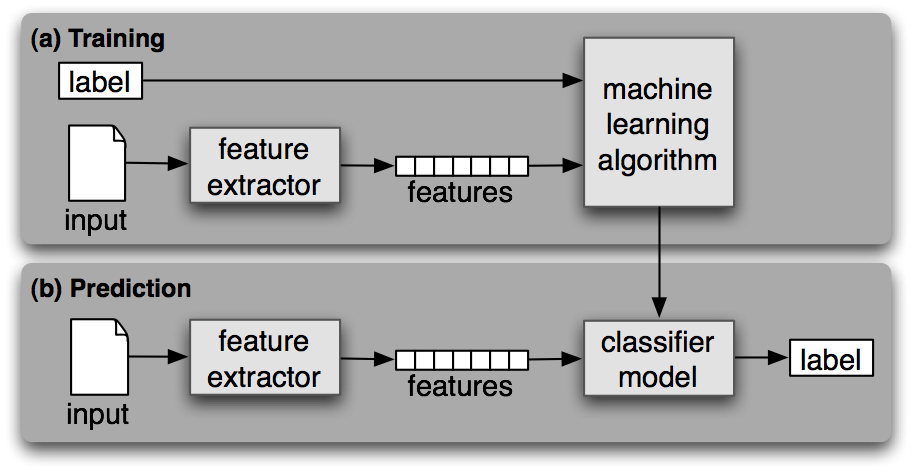
\includegraphics[scale=.8]{../Figures/mlpipeline.png} \centering
\caption{Figure Showing Workflow of Machine Learning }
\end{figure}

\section{Feature Extraction}

The first step in any machine learning task is feature extraction in which a text input is transformed into a set of attributes that characterize it. An example of a feature of a negative sentiment document may be the presence of the word \emph{terrible}. Choosing what features to use when representing a text or a document not only has a major impact on the entire classification process, but it is also arguably the most difficult phase in any natural language processing task. The reasons go to several fundamental questions on how to represent language computationally. For example, on what level should we represent a text: \emph{character-wise}, \emph{word-wise} or \emph{sentence-wise}, or even more specifically morphologically, etymologically or phonologically? Do we treat a word e.g. \emph{try} and all its morphological variations e.g. \emph{tries}, \emph{trying}, \emph{tried} similarly or differently? How to represent and model the semantics of human language computationally? Questions like these and many others are the core of natural language processing. Nevertheless, several automatic feature extraction methods have developed over the past decades that can be categorized into frequency-based or distributional, and we briefly explore some of the most common ones.

\subsection{Frequency-based Methods}

Frequency-based methods such as Bag-of-Words (BOW) and tfidf rely on number of occurrence of tokens in the text. They have been used extensively in a wide range of NLP applications, and each of them has advantages and disadvantages. 
% Representing a text computationally requires decision-making from the feature designer due to the complicated nature of human langauge language. 
\subsubsection*{Bag-of-Words Representation}

The bag-of-words (BOW) representation is the most straightforward and most intuitive
representation. It represents each document by a vector
whose component corresponds to the number of occurrences of a word in
the document.  To illustrate, the BOW vector representations of a data set of two documents (1) and (2) are shown in table \ref{tb:bow}:

\begin{enumerate}
\item The apple is better than the orange.
\item The summar is better than winter. 
\end{enumerate}




\begin{table}
\centering
\caption {Bag-of-words feature example}
\begin{tabular}{l|l|l|l|l|l|l|l|l|l|l}
 & the & apple & is & better & than & orange & summer & winter \\
Vector 1 & 2 & 1 & 1 & 1 & 1 & 1 & 0 & 0 \\
Vector 1 & 0 & 1 & 1 & 1 & 0 & 1 & 1 & 1 \\
\end{tabular}
\label {tb:bow}
\end{table}


Despite the simplicity of BOW method,  it has two main disadvantages. One major disadvantage is that BOW method pays no respect to the order of tokens in the document, and this can give similar representations to semantically different documents. For instance, the sentences \emph{the wolf eats the goat} and \emph{the goat eats the wolf} have similar vector representation as they have exact same words. Another downside to BOW is that features with high frequency are more important than those of less frequency. We can see in \ref{tb:bow} that the component corresponding to the first dimension (the) of vector 1 is bigger than in that of vector 2 because document 1 has two occurrence of the word \emph{the} while the document 2 has only one occurrence. 

To address the problem of order, several studies have attempted to count the occurrence of sentences instead of words \citep{fuhr1991probabilistic} \citep{tzeras1993automatic}. Although the sentences offer the advantage of better preserving the semantic relationship of the words, their use as features failed in practice. According to Lewis \citep{lewis1992representation}, this representation is penalized by a large number of possible combinations which leads to low and too
random frequencies. A more practical approach is representation by n-grams. It consists of breaking the text into moving sequences of $n$ consecutive tokens. For example, the trigram segmentation of the word "language" gives the following 3-grams: lan, ang, ngu, gua, uag, age. The notion of n-grams was introduced by  \citep{shannon1948mathematical}; who was interested in predicting the appearance of certain characters according to the other characters. Since then, n-grams have been used in many areas such as speech recognition and information retrieval. Using n-gram on a character-level or word-level gives a contextual representation of the text.A modification to BOW to overcome the bias of high frequency tokens result in devising a method called Term Frequency Inverse Term Frequency (tfidf). 

\subsubsection*{TFIDF Representation}

TFIDF has two main parts. Term Frequency is proportional to the frequency of the term in the document (local weighting). It can be used as is or in several variations \citep{singhal1997learning} \citep{sable2001using}.

$$t f _ { i j } = f \left( t _ { i } , d _ { j } \right)$$

$$t f _ { i j } = 1 + \log \left( f \left( t _ { i } , d _ { j } \right) \right)$$

$$ t f _ { i j } = 0.5 + 0.5 \frac { f \left( t _ { i } , d _ { j } \right) } { m a x _ { t _ { i } \in d _ { j } } f \left( t _ { i } , d _ { j } \right) }$$

where $f(t_{i},d_{j})$ is the term frequency of document $j$. Variations include logarithmic scaling of frequency counting or normalization. 

Inverse Document Frequency measures the importance of a term throughout the collection (overall weighting). A term that often appears in the document base should not have the same impact as a less frequent term. Indeed, the terms that appear in the majority of documents do not have any discriminating power to distinguish documents from each other and must, therefore, have low weightings. The IDF weighting is inversely proportional to the number of documents containing the term to be weighted. Thus, the more the term appears in several documents, the less it is discriminating and is assigned a low weighting. The IDF weighting is generally expressed as follows:

$$i d f \left( t _ { i } \right) = \log \left( \frac { N } { d f \left( t _ { i } \right) } \right)$$

where $df(t_{i})$ is the term frequency of feature $i$ and $N$ is the number of documents in the corpus.

The TFIDF weighting combines the two weightings TF and IDF in order to
provide a better approximation of the importance of a term in a
document. According to this weighting, for a term to be important in a
document, it must frequently appear in the document and rarely in other
documents. This weighting is given by the product of the local weighting
of the term in the document by its overall weighting in all the
documents of the corpus.

$$t f i d f \left( t _ { i } , d _ { j } \right) = t f _ { i j } \times \log \left( \frac { N } { d f \left( t _ { i } \right) } \right)$$

Frequency-based text representation methods explored so far, despite their usefulness in a variety of tasks in natural language processing, share sparsity as one problem in common. The number of features generated using these methods can easily exceed the tens of thousands, and that does not only negatively influence the categorization process, but it is also very computationally expensive in terms of hardware resources. In addition, the higher the dimensions of the features are, the weaker the features become. This problem is known as the \emph{curse of dimensionality} \citep{bellman2015adaptive}. To remedy this issue,  techniques, borrowed from the field of information theory and linear algebra, have been developed to reduce the feature space dimensionality without losing much information. 
% Frequency-based representation emthods, in both of its variants BOW and tfidf, drive most of search engines and recomednation systems algorithms, but they still share a critical problem of sparsity. The number of features of a data set is equal to the union of all terms in the data set, and this can be extremely large in size. Therefore, we will explore some techniques to address this issue.  
% TFC is a modification to TFIDF that overcomes the major drawback of the
% TFIDF measure, namely that the length of the documents is not taken into
% consideration by adding a normalization factor. The TFC weighting of a
% term $i$ in a document $j$ is calculated as follows:

% $$T F C _ { i j } = \frac { T F I D F \left( t _ { i } , d _ { j } \right) } { \sqrt { \sum _ { k = 1 } ^ { T } T F I D F \left( t _ { k } , d _ { j } \right) ^ { 2 } } }$$
% The use of n-grams offers the following advantages: 1) language-independent 2) Requiring no prior segmentation of the document. 3) Less sensitive to misspellings. 4) effective method to automatic language identification.

% The first challenge is how to identify words. In English, for instance, while white-space character is the indicator of words boundry, there are cases like \emph{New York} that need decision on whether or not they should be treated as one or two words. A word as being a sequence of
% characters belonging to a dictionary, or formally, as being a sequence
% of characters separated by spaces or punctuation characters. This
% definition is not valid for all languages. Indeed, languages such as
% Chinese or Japanese do not separate their words by spaces. In addition, some separators can be part of certain words (for example today,
% 127.0.0.1, potato). Another difficulty concerns the management of
% compound words (for example rainbow, potato) and acronyms (like:
% IBM, CAF, CAN, etc.). Consideration of these cases requires quite
% complex language treatments. This representation of texts excludes any
% grammatical analysis, and any notion of order between words and therefore
% semantically distant texts can have the same representation. For
% example, the sentences \texttt{the\ wolf\ eats\ the\ goat} and
% \texttt{the\ goat\ eats\ the\ wolf} is given the same representation
% despite being semantically different.

% \subsubsection{Representation by Sentences}

% Bag-of-words representation excludes any notion of order and
% the relationship between the words of a text, several studies have
% attempted to use sentences as features instead of words \citep{fuhr1991probabilistic} \citep{tzeras1993automatic}.
% The use of the sentences makes it possible to solve the problem of
% ambiguity generated by the use of the representation "bag of words." For
% example, the word \texttt{mouse} has several possible meanings while
% optical mouse and domestic mouse has no ambiguity. Although the
% sentences have the advantage of better keeping the semantics in relation
% to the words, their use as features did not lead to the expected
% results. According to Lewis \citep{lewis1992representation}, this representation is penalized
% by a large number of possible combinations which leads to low and too
% random frequencies. One solution proposed in \citep{caropreso2001learner} was to consider a
% sentence as a set of contiguous (but not necessarily ordered) words that
% appear together but do not necessarily respect grammatical rules.

% \subsubsection{Representation by lemmas or lexical roots}

% A modification to the "bag of words" is representation by lemmas or lexical roots which replaces  each word by its canonical form so that words with different
% forms (singular, plural, masculine, feminine, present, past,
% future) can have in a single form called a canonical form.
% Grouping the different forms of a word offer the advantage of reducing the dimensionality of the learning space. Indeed, in the bag-of-words representation, each form of a word is given a dimension; while with lemma representation the different forms of one word will be merged into one dimension. For example, words such as play, player, players, plays, and played will be replaced by the lemma play.


% Lemmatization and stemming are the two techniques used to find the canonical form of a word. Lemmatization uses a knowledge base containing the different inflected forms corresponding to the different possible lemmas. Thus, the inflected forms of a noun will be replaced by the singular masculine form while the infinitive form will replace the different inflected forms of a verb. Lemmatization requires the use of a dictionary of inflected forms of language as well as a grammar labeler. An efficient algorithm, named TreeTagger \citep{schmid1994probabilistic}, has been developed for thirteen different languages: German, English, French, Italian, Dutch, Spanish, Bulgarian, Russian, Greek, French Portuguese, Chinese, Swahili, and Old French. Stemming uses a knowledge base of syntactic and morphological rules and to transform words into their roots. One of the most well-known stemming algorithms for the English language is Porter's algorithm \citep{porter1980algorithm}. Lemmatization is more complicated to implement since it depends on the grammatical labelers. In addition, it is more sensitive to misspellings than stemming.

% \begin{lstlisting}[language=Python, caption=Python example]
% def stem(word):
%     Suffix_list = ["ing","ly","ed","ious",\
%                 "ies","ive","es","s","ment"]
%     for suffix in Suffix_list:
%         if word.endswith(suffix):
%             return word[:-len(suffix)]
%     return word
% \end{lstlisting}

% \subsubsection{Representation by n-grams}




% \subsubsection{Representation by concepts}



% \subsubsection{Weighting of the features}

% Co-occurrence methods such as bag-of-words have significant drawbacks, one of which is terms with higher frequency are more important than those with less frequency. Several normalization methods were developed to remove the bias towards more frequent terms. One of these methods is Term Frequency Inverse Document Frequency (TFIDF).



\subsection{Dimensionality reduction}

There are number of linguistic and non-linguistic ways to reduce the number of features in text data. Depending on the task, we can aggregate words of certain linguistic relation in concepts. For example, we replace co-hyponyms \emph{dog} and \emph{wolf} with their hypernym \emph{canine}; or \emph{vehicle} and \emph{car} with \emph{automobile}. Concepts, defined as units of knowledge, can be used as features to solve the ambiguity problem as well as the problem of synonymy. Indeed, each concept represents a unique meaning that can be expressed by several synonymous words. Similarly, a word with many meanings (senses) is found mapped to several concepts. Thus, a document containing the word \emph{vehicle} may be indexed by other words such as car or automobile. The transition from a word representation to a concept representation requires the use of semantic resources external to the content of documents such as semantic networks, thesauri, and ontologies. As a result, the performance of such a representation crucially depends on the semantic richness of the resources used in terms of the number of concepts and relationships between these concepts. 

In some cases, we may need to treat morphologically variants words similarly. For example, words such as play, player, players, plays, and played will be replaced by \emph{play}. Lemmatization and stemming are the two techniques used to find the canonical form of a word. Lemmatization uses a knowledge base containing the different inflected forms corresponding to the different possible lemmas. Thus, the inflected forms of a noun will be replaced by the singular masculine form while the infinitive form will replace the different inflected forms of a verb. Lemmatization requires the use of a dictionary of inflected forms of language as well as a grammar labeler. Stemming uses a knowledge base of syntactic and morphological rules and to transform words into their roots. One of the most well-known stemming algorithms for the English language is Porter's algorithm \citep{porter1980algorithm}. Lemmatization is more complicated to implement since it depends on the grammatical labelers. In addition, it is more sensitive to misspellings than stemming.

\begin{lstlisting}[language=Python, caption=An example of simple Stemmer Written in Python]
def stem(word):
    Suffix_list = ["ing","ly","ed","ious",\
                "ies","ive","es","s","ment"]
    for suffix in Suffix_list:
        if word.endswith(suffix):
            return word[:-len(suffix)]
    return word
\end{lstlisting}

Dimensionality reduction can also be done using probabilistic and linear algebraic techniques such as principal component analysis (PCA) and linear discriminant analysis (LDA) that aim to project highly dimensional data into lower dimension space. But we limit the discussion to only two methods: clustering and Latent Semantic Allocation. 

Clustering \citep{baker1998distributional} \citep{sable2001using} \citep{slonim2001power} can be used to reduce dimensionality. It consists of representing the documents in a new representation space other than the original one — each dimension of the new representation space groups terms that share the same meaning. Thus, the documents will no longer be represented by terms but rather by groupings of terms representing semantic concepts. This new space of representation offers the advantage of managing the synonymy since the synonymous terms will appear in the same groupings. Likewise, the fact that a term can be included in several groupings also makes it possible to manage the polysemy. Another exciting method to reduce dimensionality, proposed by \citep{deerwester1990indexing} is Latent Semantic Allocation (LSA). It uses singular value decomposition of the document $x$ term matrix to change the representation by keeping only the $k$ axes of strongest singular values. However, LSA is very expensive in terms of calculation time during learning as it relies on a matrix factorization method called Singular Value Decomposition (SVD) which runs computationally in cubic size. Likewise, with each new document, it is necessary to redo the whole grouping process.

\subsection{Distributional Method}
An alternative approach for text representation in natural language of processing is the distributional similarity. The basic idea of the distribution of similarity is to represent the meaning of a word using words which co-occurs in the same context. "You shall know a word by the company it keeps" \citep{firth1957synopsis}. For example, the words 'dog' and 'cat' have the same meaning in the following two sentences: I have a cat, I have a dog. While this idea might not be adequate to capture or account for the complexity or the sophistication of human language, it has succeeded tremendously in a variety of lexicalized NLP tasks. It has become the de facto representation method of text. The need for such a method does not only come from the need for more accurate numerical representation, but its density compared to other methods makes it less computationally expensive. Word2Vec \citep{mikolov2013distributed} and GloVe \citep{pennington2014glove} are two famous algorithms for creating word embedding. 

The intuition of word2vec is to train a classifier on a binary prediction task: “Is
word $w$ likely to show up near X?”, where $X$ is the word to which we want to find embeddings. Then, we use the weights learned by the classifier as embeddings. Skip-gram algorithm \citep{mikolov2013distributed} , first, initializes embeddings randomly. Then, it iteratively updates the embeddings of each word $w$ to be equal to the words they occur within the same context. Finally, it injects $k$ number non-neighbor words as negative examples. 

\section{Logistic Regression}

Logistic regression is a machine learning classifier that is used in a variety of learning tasks in natural language processing and computer vision. It belongs to a group of probabilistic classifiers called discriminative models which, unlike its generative counterparts like Naive Bayes classifiers, tries to distinguish the classes rather than learn to generate them. More formally, given a document $x$ and a class $y$ , logistic regressions computes the conditional probability of a class $y_i$ given its input $x_i$ $P(y|x)$. There are two types of logistic regression classifier: binary and multinomial. The binary logisitc regression is used when there are two classes of inputs to be predicted such as spam or not spam; positive or negative; malignant or benign. Multinomial or multi-class logistic regression is used when the number of predicted classes is more than two such positive, neutral or negative.

 According to \citep{jurafsky2014speech}, classification using logistic regression, like any other supervised classification algorithm, has four main components: 

\begin{list}{•}{}
 \item A feature extractor: to numerically represent language data (characters, words and sentences, etc) input $\mathbf{X}$ as feature vector $\left[x_1,x_2,\ldots,x_n \right]^T$ where $n$  represents the number of features in the input data.

\item A classification function to compute an estimation to class $\hat{y}$ via $p(y|x)$. The use of classification function determines whether the classifier is binary or multinomial. 
 
\item An objective function to minimize the error predicted label $\hat{y}$ and actual label $y$ in training examples (cross entropy)

\item An optimizer to help find the minimum of the objective function 
 (stochastic gradient descent).
 \end{list}

% Logistic regression also has two phases: training and testing. In the training phase, the goal is to find the optimal weights that best account for mapping input features $x_{i}$ to the labeled output $y_{i}$ of a subset of the data. In testing, we measure the generalizability of weights learned in the training phase on the remaining set of the data.

% Formally, the goal of logisitic regression is to learn the set of weights $\theta$ that minimizes the loss between the true $y$ labels in the training data given the input data $x$
Given a dataset of $m$ number of observations $x$ and classes $y$ $\mathcal { D } = \left\{ \left( \boldsymbol { x } ^ { ( i ) } , y ^ { ( i ) } \right) \right\} _ { i = 1 } ^ { m }$, the goal is to learn the set of optimal weights $\hat{w}$ that maximizes the log probability of predicting a class $y$ given an observation $x$

\begin{equation}
\hat{w}=\underset{w}{\operatorname{argmax}}\left[\sum_{1=i}^{m} \log P\left(y^{(i)} | x^{(i)}\right)\right]
\end{equation}

The distribution type of $P\left(y^{(i)} | x^{(i)}\right)$ determines whether the type of learning is binary or multiclass. The probability distribution of binary output is Bernoulli, while the probability distribution of multiclass output is multinomial. 

\subsection{Classification Functions}
What we have discussed so far gives us a method to numerically translate language from a form that is uniquely comprehensible to humans into a representation that a computer can understand, and can somehow capture the characteristics of human language. However, in order for the logistic regression to learn to classify, a classification function should be utilized. Depending on whether the classification task is binary or multinomial, there are two main functions used: Sigmoid and Softmax. Sigmoid function, used for binary classification, outputs 1 if an observation input (feature vector) is a member of a particular class e.g. (spam), and 0 otherwise. In other words, it calculates $P(y=1|x)$ for spam text and $P(y=0|x)$ for non-spam text. The mathematical form of the Sigmoid function or (logistic function, hence comes the name of the classifier) is as follow:

$$Sig ( x ) = \frac { 1 } { 1 + e ^ { - (w \cdot x +b)} }$$ 

where $x$ represent the input vector, $w$ is the learned weights, and $b$ is the bias term or the intercept of the linear equation. One mathematical property of the Sigmoid function is that it maps any input between 0 and 1, and to make it as probability we need to make the sum of $P(y=1)$ and $P(y=0)$ equals to 1. 

$$ P ( y = 1 ) = \sigma ( w \cdot x + b ) $$
$$ P ( y = 0 ) = 1 - \sigma ( w \cdot x + b ) $$

Now to make a decision, the classifier declares an observation input as \emph{Yes} (if it is a member of class spam) if the probability is greater than a certain threshold, say 0.5, and declares an observation input as \emph{No} otherwise. 

$$  \hat { y } = \left\{ \begin{array} { l l } { 1 } & { \text { if } P ( y = 1 | x ) > 0.5 } \\ { 0 } & { \text { otherwise } } \end{array} \right.  $$


In the case of multinomial classification, the logic remains the same except for the classification function where Softmax is used rather than Sigmoid. Softmax works on normalizing the prediction of an observation by the values of all other classes in order to produce valid probability distribution. 

$$p ( y = i | x ) = \frac { e ^ { w _ { i } \cdot x + b _ { i } } } { \sum _ { j = 1 } ^ { k } e ^ { w _ { j } \cdot x + b _ { j } } }$$



\subsection{Objective Functions}

During the learning process, we need to answer the question of \emph{how correct is the estimated output of $\hat{y}$ of classifier from the true output $y$?}. Thus our objective \emph{function} is to minimize the difference between the estimated output and the true one such that the weights learned during this minimization process are, hopefully,  generalizable enough to correctly label observations unseen in the training phase. So we can imagine an objective function to be a difference between the $\hat{y}$ and $y$ i.e. $\left | \hat{y} - y \right |$, but for mathematical convenience we need a non-convex objective function (or also commonly referred to as loss function)  that can be easily optimized. Thus, we use maximum likelihood estimation. 

Binary classification can be seen as Bernoulli distribution since the outcome is either 0 or 1. More formally, the probability of predicting class $y$ given input $x$ is  $p ( y | x ) = \hat { y } ^ { y } ( 1 - \hat { y } ) ^ { 1 - y }$. Minimizing the probability is the same as maximizing the negative log likelihood:
 $$L _ { C E } ( \hat { y } , y ) = - \log p ( y | x ) = - [ y \log \hat { y } + ( 1 - y ) \log ( 1 - \hat { y } ) ]$$

Finally, by plugging in the value of $\hat{y}$ we get:
$$ L _ { C E } ( w , b ) = - \frac { 1 } { m } \sum _ { i = 1 } ^ { m } y ^ { ( i ) } \log \sigma \left( w \cdot x ^ { ( i ) } + b \right) + \left( 1 - y ^ { ( i ) } \right) \log \left( 1 - \sigma \left( w \cdot x ^ { ( i ) } + b \right) \right) $$, where $m$ is the number of training examples.

On the other hand, multinomial classification uses the same process except that it uses a different classification function \emph{softmax} and hence has different (multinomial) distribution. So the loss function for a single example $x$ is the sum of the logs of the $K$ output classes:
$$ L _ { C E } ( \hat { y } , y ) = - \sum _ { k = 1 } ^ { K } 1 \{ y = k \} \log \frac { e ^ { w _ { k } \cdot x + b _ { k } } } { \sum _ { j = 1 } ^ { K } e ^ { w _ { j } \cdot x + b _ { j } } } $$

\subsection{Optimization}

The objective functions derived in the previous section is optimized using numerical methods. Several algorithms are used for this purpose such as Stochastic Gradient Descent, that uses first derivative (gradient) information to find a minimum of a function; Newton-Raphson algorithm uses Second derivative information to find a minimum of a function. Discussing the details of how these algorithms work and the mathematical derivation of gradients is beyond the scope of this work. Interested readers are referred to \citep{jurafsky2014speech} for more details on the derivation of Stochastic Gradient Descent. 

\section{Evaluation Metrics}
\subsection{Confusion Matrix}

A confusion matrix is a method to visualize the results of a classification algorithm. For the binary classification, the algorithm can be used to predict whether a test sample is either 0, or 1. As a way to measure how well the algorithm performs, we can count four different metrics, here 1 defined as positive and 0 defined as negative:

\begin{enumerate}

\item True positive (TP), the algorithm classifies 1 where the correct class is 1.
\item False positive (FP), the algorithm classifies 1 where the correct class is 0.
\item True negative (TN), the algorithm classifies 0 where the correct class is 0.
\item False negative (FN), the algorithm classifies 0 where the correct class is 1.

\end{enumerate}

\begin{figure}[hbtp]
\caption{Confusion Matrix Example}
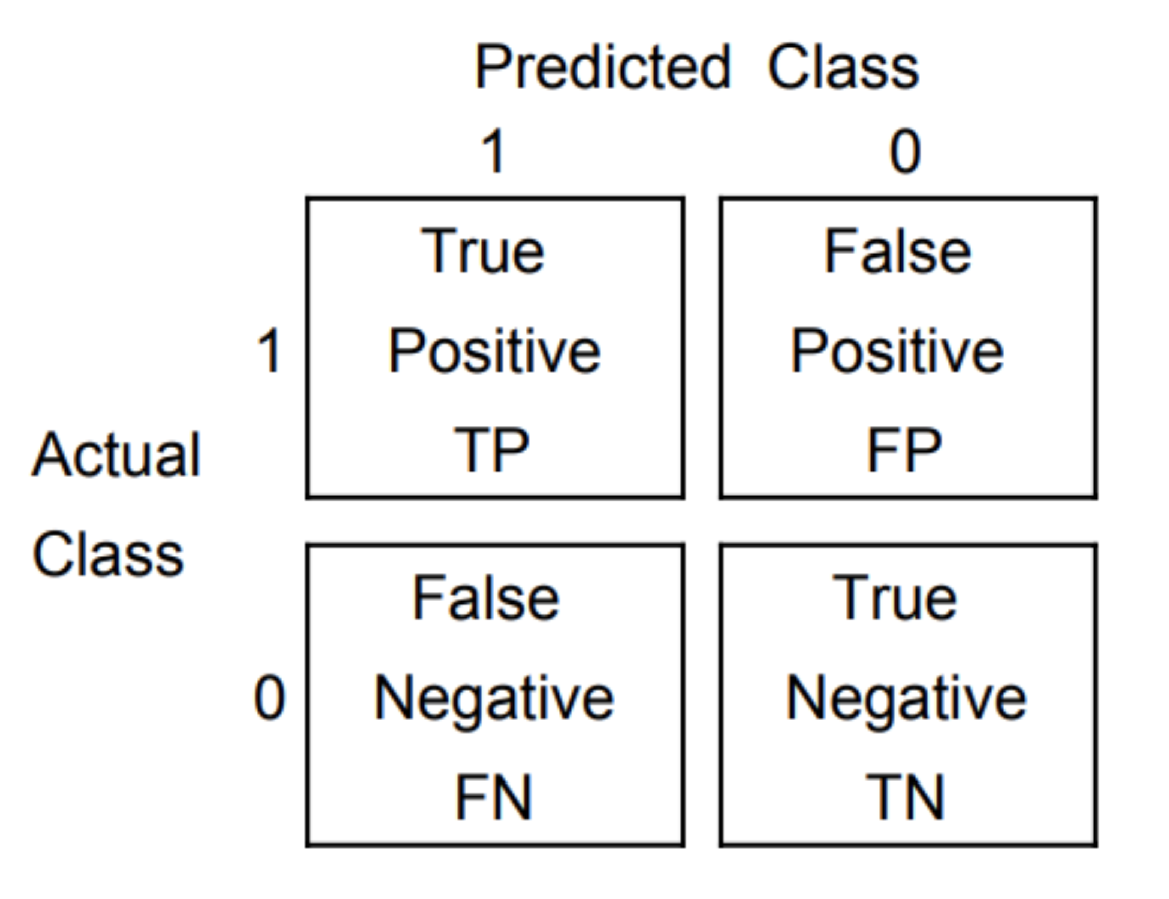
\includegraphics[scale=.5]{../Figures/Confuse_Mat_Example.png}\centering
\end{figure}

\subsection{Precision, Recall and F-Score}

Precision and Recall are two popular measurement to evaluate the performance of supervised classification methods. Precision is defined as:

$$\text { Precision } = \frac { True Postive } { True Postive + False Positive }$$

, recall defined as:

$$\text { Recall } = \frac { True Postive } { True Postive + False Negative }$$

and F-score is the harmonic mean of both precision and recall:

$$F _ { 1 } = 2 \cdot \frac { \text { precision } \cdot \text { recall } } { \text { precision } + \text { recall } }$$

A classifier with high precision means it classifies almost no inputs as positive unless they are positive. A classifier with high recall, on the other hand, would mean that  it misses almost no positive values. 
\section{Conclusion}

In this chapter, we briefly introduced some fundamental topics of Machine Learning theory required for natural language processing supervised classification tasks. We discussed two commonly used numerical methods to represent text computationally and their variants, Frequency-based methods: Bag-of word models (BoW) and Term Frequency - Inverse Document Frequency (tfidf), and Distributional similarity methods. Besides, we reviewed some techniques to reduce the dimensionality of feature space to reduce the complexity of the training and save computational resources. Finally, we covered how logistic regression as a probabilistic algorithm can be used for binary or multinomial classification along with the evaluation metrics used to gauge its performance. In the next two chapters, we show the use of multinomial logistic regression classifier on two novel tasks in natural language processing: grammatical difficulty categorization of English sentences and automatic reading comprehension. We also explore how logistic regression can be used in a semi-supervised manner to work on tasks with limited data. 